% !TeX program = xelatex
% 从 教学课件/习题课模板/习题课模板.tex 复制后填入本课内容。
% 来源A：教学课件/必修一/提取自教材帮.pdf，PDF第1—8页，书页154—161。
% 来源B：教学课件/必修一/提取自教材帮(1).pdf，PDF第1页，书页100。
\ifdefined\PrintVersion
  \PassOptionsToClass{handout}{ctexbeamer}
\fi
\documentclass[UTF8,10pt,aspectratio=169]{ctexbeamer}
\usepackage{amsmath,amssymb}
\usepackage{tikz}
\usetikzlibrary{calc,arrows.meta,positioning,shapes.geometric}
\usepackage{newtxtext,newtxmath}
\usetheme{default}
\usecolortheme{default}
\usefonttheme{serif}
\setbeamertemplate{navigation symbols}{}
\setbeamertemplate{footline}[frame number]

\newcommand{\LessonTitle}{指数函数与复合函数}
\newcommand{\LessonSubtitle}{高一数学\quad 教材帮习题课}
\newcommand{\LessonInfo}{2026年11月5日}
\newcommand{\PageHeading}[1]{\begin{center}{\Large\bfseries #1}\end{center}\vspace{0.2cm}}
\newcommand{\Answer}[1]{\par\vspace{0.2cm}\textbf{【答案】}#1}
\newcommand{\Analysis}[1]{\par\vspace{0.2cm}\textbf{【详解】}#1}
\newcommand{\Choices}[4]{\par\vspace{0.2cm}\begin{tabular}{@{}p{0.47\textwidth}p{0.47\textwidth}@{}}A. #1 & B. #2 \\[0.15cm] C. #3 & D. #4\end{tabular}}

\begin{document}
\begin{frame}[label=cover]
  \begin{center}
    {\Large\bfseries \LessonTitle}\par\vspace{0.5cm}
    {\large \LessonSubtitle}\par\vspace{0.4cm}
    \LessonInfo
  \end{center}
  \vspace{0.4cm}
  \textbf{学习目标：}
  \begin{enumerate}
    \item 结合图象和单调性比较指数幂，解指数方程与不等式。
    \item 换元时保留范围，判断复合函数的单调性与最值。
    \item 利用奇偶性、对称性及参数条件完成综合问题。
  \end{enumerate}
\end{frame}

% !TeX encoding = UTF-8
% 来源A：教学课件/必修一/提取自教材帮.pdf，第1--3页，书页154--156。
% 本文件仅含frame；供固定习题课模板的主文件input。

% 来源：A第1页／书154页，例8（2026·湖南省长沙市雅礼中学期中）。
% 目标：指数图象过定点；方法：令指数为0或平移(0,1)；易错：漏掉纵向平移；难度：基础；评价：说明x=3为何与底数无关。
\begin{frame}[t,label=A08q]
  \PageHeading{例8：过定点问题}
  函数 $y=a^{x-3}+3\ (a>0,\ a\ne1)$ 的图象过定点
  \underline{\hspace{2cm}}。
  \par\vspace{0.2cm}（2026·湖南省长沙市雅礼中学期中）
  \pause
  \Answer{$(3,4)$。}
  \Analysis{方法一：$y=a^x$ 的图象过定点 $(0,1)$。
  向右平移3个单位、再向上平移3个单位，得到定点 $(3,4)$。}
  \par\vspace{0.2cm}
  方法二：令 $x-3=0$，得 $x=3$。由 $a^0=1$，得 $y=1+3=4$。
\end{frame}

% 来源：A第1页／书154页，解题通法“指数型函数图象过定点问题的思路”。
% 目标：概括定点结构；方法：指数为0；易错：把-c写成c；难度：基础；评价：写出定点并核对参数条件。
\begin{frame}[t,label=A08m]
  \PageHeading{解题通法：指数型函数图象过定点}
  指数函数 $y=a^x\ (a>0,\ a\ne1)$ 的图象过定点 $(0,1)$。
  \par\vspace{0.3cm}
  对于 $y=k\,a^{x+c}+b\ (k\ne0,\ a>0,\ a\ne1)$，怎样找定点？
  \pause
  \Analysis{令 $x+c=0$，得 $x=-c$；此时 $y=k+b$。}
  \[
    \boxed{\text{定点为 }(-c,k+b).}
  \]
  \par\vspace{0.2cm}
  关键是利用 $a^0=1$，让函数值不再随底数 $a$ 改变。
\end{frame}

% 来源：A第1页／书154页，例9（多选题）。
% 目标：绝对值指数图象与条件转化；方法：分段单调性、均值不等式；易错：把a<c直接当函数值同序；难度：提高；评价：逐项给出依据或反例。
\begin{frame}[t,label=A09q]
  \PageHeading{例9：图象的应用与数形结合}
  【多选题】已知 $f(x)=|2^x-1|$，当 $a<b<c$ 时，有
  $f(a)>f(c)>f(b)$。则下列结论正确的为（\quad）。
  \Choices{$a+c<0$}{$b+c<0$}{$2^a+2^c>2$}{$2^b+2^c>2$}
  \pause
  \Answer{AD。}
  \Analysis{先由图象及单调性确定 $a<0<c$，再去掉绝对值。
  条件转化与选项判断见续页。}
\end{frame}

% 来源：A第1页／书154页，例9解析与图4.2-7。图象按f(x)=|2^x-1|重绘。
% 目标：判定a,c的符号；方法：反证及分段单调；易错：遗漏c=0；难度：提高；评价：能说明a>=0和c<=0均矛盾。
\begin{frame}[t,label=A09a]
  \PageHeading{例9详解：先确定 $a,c$ 的符号}
  已知 $a<b<c$，$f(a)>f(c)>f(b)$，且 $f(x)=|2^x-1|$。
  \begin{columns}[T]
    \begin{column}{0.40\textwidth}
      \begin{center}
      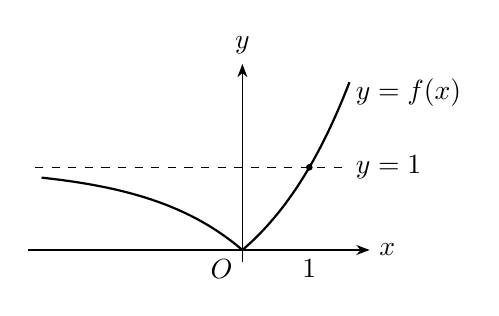
\begin{tikzpicture}[x=0.85cm,y=1.05cm]
        \draw[-{Stealth}] (-3.2,0)--(1.9,0) node[right] {$x$};
        \draw[-{Stealth}] (0,-0.15)--(0,2.25) node[above] {$y$};
        \draw[dashed] (-3.1,1)--(1.55,1) node[right] {$y=1$};
        \draw[thick,domain=-3:0,samples=70] plot (\x,{1-pow(2,\x)});
        \draw[thick,domain=0:1.6,samples=70] plot (\x,{pow(2,\x)-1});
        \node[below left] at (0,0) {$O$};
        \fill (1,1) circle (1.2pt);
        \node[below] at (1,0) {$1$};
        \node[right] at (1.55,1.9) {$y=f(x)$};
      \end{tikzpicture}
      \end{center}
      $(-\infty,0]$ 上严格递减；
      \par $[0,+\infty)$ 上严格递增。
    \end{column}
    \begin{column}{0.57\textwidth}
      \pause
      \Analysis{若 $a\ge0$，则 $f(a)<f(c)$，矛盾。
      \par 若 $c<0$，由 $b<c$ 得 $f(b)>f(c)$，矛盾。
      \par 若 $c=0$，则 $f(c)=0\le f(b)$，仍矛盾。
      \par 因此 $a<0<c$。}
      \[
        1-2^a>2^c-1
        \quad\Longrightarrow\quad 2^a+2^c<2.
      \]
      所以C错误。
    \end{column}
  \end{columns}
\end{frame}

% 来源：A第1页／书154页，例9解析。补写B的具体反例，补齐原解b=0情形。
% 目标：论证A、D及否定B；方法：均值不等式、分b符号；易错：用“大于均值”误判和的上界；难度：提高；评价：每步不等式方向与条件齐全。
\begin{frame}[t,label=A09b]
  \PageHeading{例9详解：判断A、B、D}
  沿用条件 $a<b<c$、$f(a)>f(c)>f(b)$，已得 $a<0<c$、$2^a+2^c<2$。
  \pause
  \Analysis{由
  $2\sqrt{2^{a+c}}\le2^a+2^c<2$，得 $2^{a+c}<1$，故 $a+c<0$，A正确。}
  \par\vspace{0.2cm}
  对D：若 $b\ge0$，则 $c>b\ge0$，所以 $2^b+2^c>2$。
  \par 若 $b<0$，则 $f(c)>f(b)$ 给出
  \[
    2^c-1>1-2^b\quad\Longrightarrow\quad2^b+2^c>2.
  \]
  因此D正确。
  \par\vspace{0.2cm}
  对B：取 $a=-2,b=0,c=\tfrac12$，有
  $f(a)=\tfrac34>\sqrt2-1>0=f(b)$，但 $b+c=\tfrac12>0$。
  所以B错误。
\end{frame}

% 来源：A第1--2页／书154--155页，例10（教材改编P117例3）。
% 目标：识别同底、同指数、均不同结构；方法：单调性与中间量；易错：负指数比较底数时方向；难度：基础至中等；评价：三问给方向且说依据。
\begin{frame}[t,label=A10q]
  \PageHeading{例10：比较大小}
  比较下列各题中两个值的大小。
  \par\vspace{0.2cm}
  （1）$\left(\dfrac57\right)^{-1.8}$，$\left(\dfrac57\right)^{-2.5}$；
  \par\vspace{0.2cm}
  （2）$\left(\dfrac23\right)^{-0.5}$，$\left(\dfrac34\right)^{-0.5}$；
  \par\vspace{0.2cm}
  （3）$0.2^{0.3}$，$0.3^{0.2}$。
  \par\vspace{0.2cm}（教材改编：P117例3）
  \pause
  \Answer{（1）$<$；（2）$>$；（3）$<$。}
\end{frame}

% 来源：A第1页／书154页，例10（1）及“结构化思维解题”。
% 目标：同底比较；方法：指数函数单调性；易错：0<a<1仍按指数同序；难度：基础；评价：明确底数范围再比较指数。
\begin{frame}[t,label=A10a1]
  \PageHeading{例10（1）：底数相同}
  比较 $\left(\dfrac57\right)^{-1.8}$ 与 $\left(\dfrac57\right)^{-2.5}$。
  \pause
  \Analysis{因为 $0<\dfrac57<1$，函数 $y=\left(\dfrac57\right)^x$ 在 $\mathbb R$ 上严格递减。
  又 $-1.8>-2.5$，所以}
  \[
    \boxed{\left(\frac57\right)^{-1.8}<\left(\frac57\right)^{-2.5}.}
  \]
  \par\vspace{0.3cm}
  \textbf{结构识别：}底数相同，直接利用指数函数的单调性。
\end{frame}

% 来源：A第1--2页／书154--155页，例10（2）方法1及图4.2-8。图按真实指数函数重绘。
% 目标：同指数比较的图象解释；方法：比较负半轴上两指数图象；易错：“底大图低”不限定x；难度：中等；评价：说明比较点在x=-0.5<0。
\begin{frame}[t,label=A10a2g]
  \PageHeading{例10（2）：观察指数函数图象}
  比较 $\left(\dfrac23\right)^{-0.5}$ 与 $\left(\dfrac34\right)^{-0.5}$。
  \begin{columns}[T]
    \begin{column}{0.45\textwidth}
      \begin{center}
      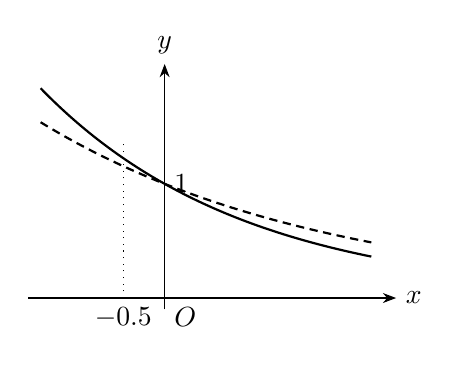
\begin{tikzpicture}[x=1.05cm,y=1.45cm]
        \draw[-{Stealth}] (-1.65,0)--(2.8,0) node[right] {$x$};
        \draw[-{Stealth}] (0,-0.1)--(0,2.05) node[above] {$y$};
        \draw[thick,domain=-1.5:2.5,samples=70] plot (\x,{pow(2/3,\x)});
        \draw[thick,densely dashed,domain=-1.5:2.5,samples=70] plot (\x,{pow(3/4,\x)});
        \draw[dotted] (-0.5,0)--(-0.5,1.35);
        \node[below] at (-0.5,0) {$-0.5$};
        \node[below right] at (0,0) {$O$};
        \node[right] at (0,1) {$1$};
      \end{tikzpicture}
      \end{center}
      实线：$y=\left(\dfrac23\right)^x$；
      \par 虚线：$y=\left(\dfrac34\right)^x$。
    \end{column}
    \begin{column}{0.52\textwidth}
      \pause
      \Analysis{在同一坐标系中画出两函数图象。
      \par 当 $x=-0.5$ 时，$y=(2/3)^x$ 的图象在 $y=(3/4)^x$ 的图象上方，所以}
      \[
        \left(\frac23\right)^{-0.5}>\left(\frac34\right)^{-0.5}.
      \]
      本题在负半轴比较，不能脱离 $x$ 的范围套用图象口诀。
    \end{column}
  \end{columns}
\end{frame}

% 来源：A第2页／书155页，例10（2）方法2。
% 目标：用幂函数严谨比较；方法：先开平方再取倒数；易错：正数取倒数忘记反向；难度：基础；评价：说清两次比较的方向。
\begin{frame}[t,label=A10a2p]
  \PageHeading{例10（2）：构造幂函数}
  比较 $\left(\dfrac23\right)^{-0.5}$ 与 $\left(\dfrac34\right)^{-0.5}$。
  \pause
  \Analysis{函数 $y=x^{0.5}$ 在 $(0,+\infty)$ 上严格递增，而 $\dfrac23<\dfrac34$，故}
  \[
    \left(\frac23\right)^{0.5}<\left(\frac34\right)^{0.5}.
  \]
  两边都是正数，取倒数后不等号反向：
  \[
    \left(\frac23\right)^{-0.5}
    =\frac1{(2/3)^{0.5}}
    >\frac1{(3/4)^{0.5}}
    =\left(\frac34\right)^{-0.5}.
  \]
\end{frame}

% 来源：A第2页／书155页，例10（3）方法1及中间量批注。
% 目标：底数指数均不同时引入中间量；方法：0.2^0.2或0.3^0.3；易错：只比较底数或指数；难度：中等；评价：每段比较都指明函数及单调性。
\begin{frame}[t,label=A10a3i]
  \PageHeading{例10（3）：引入中间量}
  比较 $0.2^{0.3}$ 与 $0.3^{0.2}$。
  \pause
  \Analysis{幂函数 $y=x^{0.2}$ 在 $[0,+\infty)$ 上严格递增，
  指数函数 $y=0.2^x$ 在 $\mathbb R$ 上严格递减。因此}
  \[
    0.2^{0.3}<\underbrace{0.2^{0.2}}_{\text{中间量}}<0.3^{0.2}.
  \]
  \par\vspace{0.3cm}
  也可引入 $0.3^{0.3}$：先利用 $y=x^{0.3}$ 递增，再利用 $y=0.3^x$ 递减，得
  \[
    0.2^{0.3}<\underbrace{0.3^{0.3}}_{\text{中间量}}<0.3^{0.2}.
  \]
\end{frame}

% 来源：A第2页／书155页，例10（3）方法2、方法3。
% 目标：转化同指数或整体乘方；方法：同写成0.1次幂或比较10次幂；易错：忽略正值条件；难度：中等；评价：能说明乘方不改变比较方向。
\begin{frame}[t,label=A10a3p]
  \PageHeading{例10（3）：转化为同指数或乘方}
  需要比较的两个数为正数 $0.2^{0.3}$ 与 $0.3^{0.2}$。
  \pause
  \Analysis{方法二：转化为同指数。}
  \[
    0.2^{0.3}=(0.2^3)^{0.1}=0.008^{0.1},\qquad
    0.3^{0.2}=(0.3^2)^{0.1}=0.09^{0.1}.
  \]
  由 $0.008<0.09$，以及 $y=x^{0.1}$ 在 $[0,+\infty)$ 上严格递增，
  得 $0.2^{0.3}<0.3^{0.2}$。
  \par\vspace{0.2cm}
  方法三：比较10次幂。
  \[
    (0.2^{0.3})^{10}=0.2^3=0.008
    <0.09=0.3^2=(0.3^{0.2})^{10}.
  \]
  因 $y=x^{10}$ 在 $[0,+\infty)$ 上严格递增，仍得 $0.2^{0.3}<0.3^{0.2}$。
\end{frame}

% 来源：A第1--2页／书154--155页，“学神题”结构图及解题通法三类。
% 目标：形成比较策略；方法：结构分类；易错：未判断底数范围便比较；难度：基础；评价：面对新式子先说结构再选方法。
\begin{frame}[t,label=A10m]
  \PageHeading{解题通法：指数幂大小比较的三种类型}
  \textbf{1. 底数相同，指数不同。}
  \par 先看底数大于1还是介于0与1，再用指数函数单调性。
  \pause
  \par\vspace{0.35cm}
  \textbf{2. 底数不同，指数相同。}
  \par 可构造幂函数；也可比较不同底数指数函数的图象，注意指数所在范围。
  \par\vspace{0.35cm}
  \textbf{3. 底数不同，指数也不同。}
  \par 尝试引入中间量（常用0、1），或转化为同底数、同指数再比较。
  \par 必要时比较两个正数的同次幂，并说明所用幂函数的单调性。
\end{frame}

% 来源：A第2页／书155页，练变式4（2026·河南省洛阳市期末）；原图M=2^a，a为正指数。
% 目标：中间量与同底同指数结合；方法：用1隔开M，再串联比较N,P；易错：误录M=2^{-a}或遗漏N的负号；难度：中等；评价：写出完整比较链。
\begin{frame}[t,label=AV04q]
  \PageHeading{练变式4：比较三个指数幂}
  已知实数 $a,b,c$ 满足 $0<a<b<c<1$，且
  \[
    M=2^a,\qquad N=5^{-b},\qquad P=\left(\frac17\right)^c.
  \]
  则 $M,N,P$ 的大小关系为（\quad）。
  \Choices{$M>N>P$}{$M>P>N$}{$N>P>M$}{$N>M>P$}
  \par\vspace{0.2cm}（2026·河南省洛阳市期末）
  \pause
  \Answer{A。}
  \Analysis{$M>1>N$；又因 $0<b<c$，
  $N=5^{-b}>7^{-b}>7^{-c}=P$。故 $M>N>P$。}
\end{frame}

% 来源：A第2页／书155页，例11。
% 目标：解指数方程；方法：同底和换元；易错：指数法则与换元正值；难度：基础；评价：分别辨认结构并给出解。
\begin{frame}[t,label=A11q]
  \PageHeading{例11：解简单的指数方程}
  解下列方程。
  \par\vspace{0.25cm}
  （1）$81\times3^{2x}=\left(\dfrac19\right)^{x+2}$；
  \par\vspace{0.25cm}
  （2）$2^{2x+2}+3\times2^x-1=0$。
  \pause
  \Answer{（1）$x=-2$；（2）$x=-2$。}
  \Analysis{（1）化为同底的指数式；（2）令 $t=2^x>0$，先解关于 $t$ 的方程。}
\end{frame}

% 来源：A第2页／书155页，例11（1）解析。
% 目标：同底比较指数；方法：81=3^4,1/9=3^{-2}；易错：右边指数乘法漏括号；难度：基础；评价：两边指数变形正确并检验。
\begin{frame}[t,label=A11a1]
  \PageHeading{例11（1）详解：化为同底}
  解方程 $81\times3^{2x}=\left(\dfrac19\right)^{x+2}$。
  \pause
  \Analysis{因为 $81=3^4$，$\dfrac19=3^{-2}$，原方程等价于}
  \[
    3^{2x+4}=3^{-2(x+2)}.
  \]
  函数 $y=3^x$ 在 $\mathbb R$ 上严格递增，同底数幂相等时指数相等：
  \[
    2x+4=-2(x+2)\quad\Longrightarrow\quad x=-2.
  \]
  代入原方程，两边都为1，故解为 $x=-2$。
\end{frame}

% 来源：A第2页／书155页，例11（2）解析与易错批注。
% 目标：换元处理指数二次式；方法：t=2^x>0；易错：保留负t或把2^{2x+2}写成(2^x)^2+4；难度：基础；评价：正确舍负根并回代。
\begin{frame}[t,label=A11a2]
  \PageHeading{例11（2）详解：换元后记住范围}
  解方程 $2^{2x+2}+3\times2^x-1=0$。
  \pause
  \Analysis{原方程可写成 $4(2^x)^2+3\cdot2^x-1=0$。
  令 $t=2^x>0$，则}
  \[
    4t^2+3t-1=(4t-1)(t+1)=0.
  \]
  得 $t=\dfrac14$ 或 $t=-1$。由于 $t>0$，舍去 $t=-1$。
  \[
    2^x=\frac14=2^{-2}\quad\Longrightarrow\quad x=-2.
  \]
  换元要保留 $t$ 的范围，解出 $t$ 后还要回到 $x$。
\end{frame}

% 来源：A第2页／书155页，解题通法：同底型、可换元型。
% 目标：概括指数方程解法；方法：同底/换元；易错：只得到t就结束；难度：基础；评价：完整叙述两步转化。
\begin{frame}[t,label=A11m]
  \PageHeading{解题通法：指数方程}
  \textbf{1. 同底型。}
  \par 把方程两边化为 $a^{f(x)}=a^{g(x)}\ (a>0,\ a\ne1)$。
  \par 利用指数函数的单调性，得到 $f(x)=g(x)$，再解方程。
  \pause
  \par\vspace{0.45cm}
  \textbf{2. 可换元型。}
  \par 若方程可写成 $F(a^x)=0$，则令 $t=a^x>0$。
  \par 先解 $F(t)=0$，舍去不满足范围的 $t$，再由 $a^x=t$ 求 $x$。
  \par\vspace{0.3cm}
  核查：指数运算是否正确，换元范围是否保留，是否已经回到原未知数。
\end{frame}

% 来源：A第2页／书155页，练变式5（1）（2026·上海市建平中学月考）。
% 目标：同底指数方程迁移；方法：4^{3x}=2^{6x}；易错：3x与底数4对应的2漏乘；难度：基础；评价：指数相等式正确。
\begin{frame}[t,label=AV05q1]
  \PageHeading{练变式5（1）：化为同底}
  方程 $2^{-x+2}=4^{3x}$ 的解集是\underline{\hspace{2.3cm}}。
  \par\vspace{0.2cm}（2026·上海市建平中学月考）
  \pause
  \Answer{$\left\{\dfrac27\right\}$。}
  \Analysis{原方程等价于 $2^{-x+2}=2^{6x}$。
  由指数函数 $y=2^x$ 的单调性，得}
  \[
    -x+2=6x\quad\Longrightarrow\quad x=\frac27.
  \]
\end{frame}

% 来源：A第2页／书155页，练变式5（2）。
% 目标：指数二次方程迁移；方法：t=2^x>0；易错：把t=2,8当成x；难度：基础；评价：解集回代为1,3。
\begin{frame}[t,label=AV05q2]
  \PageHeading{练变式5（2）：换元求解}
  方程 $4^x-10\cdot2^x+16=0$ 的解集是\underline{\hspace{2.3cm}}。
  \pause
  \Answer{$\{1,3\}$。}
  \Analysis{令 $t=2^x>0$，因 $4^x=(2^x)^2$，得到}
  \[
    t^2-10t+16=(t-2)(t-8)=0.
  \]
  两个根 $t=2,8$ 均满足 $t>0$。
  \[
    2^x=2\text{ 或 }2^x=8\quad\Longrightarrow\quad x=1\text{ 或 }x=3.
  \]
\end{frame}

% 来源：A第3页／书156页，例12。
% 目标：指数不等式；方法：同底、按底数范围分类；易错：0<a<1时方向反转；难度：基础至中等；评价：三问写解集并标明分类条件。
\begin{frame}[t,label=A12q]
  \PageHeading{例12：解指数不等式}
  求满足下列条件的 $x$ 的取值范围。
  \par\vspace{0.2cm}
  （1）$3^{x-1}>9^x$；
  \par\vspace{0.2cm}
  （2）$0.2^x<25$；
  \par\vspace{0.2cm}
  （3）$a^{-5x}>a^{x+7}\ (a>0,\ a\ne1)$。
  \pause
  \Answer{（1）$(-\infty,-1)$；（2）$(-2,+\infty)$；
  \par （3）$a>1$ 时为 $(-\infty,-\tfrac76)$；
  $0<a<1$ 时为 $(-\tfrac76,+\infty)$。}
\end{frame}

% 来源：A第3页／书156页，例12（1）（2）解析。
% 目标：不同底数化同底；方法：9^x=3^{2x},25=0.2^{-2}；易错：第二问比较指数时不反向；难度：基础；评价：底数范围与不等号一致。
\begin{frame}[t,label=A12a1]
  \PageHeading{例12（1）（2）详解}
  （1）$3^{x-1}>9^x$；\qquad（2）$0.2^x<25$。
  \pause
  \Analysis{（1）$9^x=3^{2x}$，函数 $y=3^x$ 严格递增，所以}
  \[
    x-1>2x\quad\Longrightarrow\quad x<-1.
  \]
  \par\vspace{0.3cm}
  （2）$25=0.2^{-2}$，而 $0<0.2<1$，函数 $y=0.2^x$ 严格递减，所以
  \[
    0.2^x<0.2^{-2}\quad\Longrightarrow\quad x>-2.
  \]
\end{frame}

% 来源：A第3页／书156页，例12（3）解析及“底数范围不确定”批注。
% 目标：含参底数分类；方法：a>1与0<a<1两类；易错：只解一类或a=1未排除；难度：中等；评价：分类不漏，指数不等式方向正确。
\begin{frame}[t,label=A12a2]
  \PageHeading{例12（3）详解：按底数范围分类}
  解 $a^{-5x}>a^{x+7}\ (a>0,\ a\ne1)$。
  \pause
  \Analysis{当 $a>1$ 时，函数 $y=a^x$ 严格递增，因此}
  \[
    -5x>x+7\quad\Longrightarrow\quad x<-\frac76.
  \]
  当 $0<a<1$ 时，函数 $y=a^x$ 严格递减，因此
  \[
    -5x<x+7\quad\Longrightarrow\quad x>-\frac76.
  \]
  先分清底数范围，再决定比较指数时是否改变不等号方向。
\end{frame}

% 来源：A第3页／书156页，解题通法“指数不等式的三种类型及求解方法”。
% 目标：不等式结构分类；方法：同底、常数化底、同指数比底；易错：除以可能非正量（本处指数式恒正）；难度：基础至中等；评价：方法前提说完整。
\begin{frame}[t,label=A12m]
  \PageHeading{解题通法：指数不等式的三种类型}
  \textbf{1. $a^{u(x)}>a^{v(x)}$。}
  \par 利用 $y=a^x$ 的单调性；底数范围不确定时，分 $a>1$ 与 $0<a<1$。
  \pause
  \par\vspace{0.3cm}
  \textbf{2. $a^x>b$。}
  \par 当 $b>0$ 时，先把 $b$ 化成以 $a$ 为底的幂，再比较指数。
  \par 若 $b\le0$，由 $a^x>0$ 可直接判断，不强行化同底。
  \par\vspace{0.3cm}
  \textbf{3. $a^x>b^x$。}
  \par 可化为同底数幂比较，或观察两指数函数图象。例如
  \[
    2^x>3^x\ \Longleftrightarrow\ \left(\frac23\right)^x>1
    \ \Longleftrightarrow\ x<0.
  \]
\end{frame}

% 来源：A第3页／书156页，练变式6。分段原文已核：x<0为(1/2)^x-7，x>=0为sqrt(x)。
% 目标：分段函数不等式；方法：各段解不等式并交分段范围；易错：漏-7或把sqrt(x)录成x、漏端点0；难度：中等；评价：先交后并且0保留。
\begin{frame}[t,label=AV06q]
  \PageHeading{练变式6：分段函数不等式}
  已知函数
  \[
    f(x)=\begin{cases}
      \left(\dfrac12\right)^x-7,&x<0,\\[1mm]
      \sqrt{x},&x\ge0.
    \end{cases}
  \]
  若 $f(a)<1$，则实数 $a$ 的取值范围是（\quad）。
  \Choices{$(-\infty,-3)$}{$(1,+\infty)$}{$(-3,1)$}{$(-\infty,-3)\cup(1,+\infty)$}
  \pause
  \Answer{C，即 $(-3,1)$。}
\end{frame}

% 来源：A第3页／书156页，练变式6；此页为独立补全解析，原页仅题目、答案索引。
% 目标：完整核验分段解集；方法：两段分别交范围；易错：直接把a>-3与a<1相交而无分段理由；难度：中等；评价：写出(-3,0)与[0,1)再合并。
\begin{frame}[t,label=AV06a]
  \PageHeading{练变式6详解：每段求解后再合并}
  已知 $f(x)=(1/2)^x-7\ (x<0)$，$f(x)=\sqrt{x}\ (x\ge0)$，求 $f(a)<1$。
  \pause
  \Analysis{当 $a<0$ 时，}
  \[
    \left(\frac12\right)^a-7<1
    \ \Longleftrightarrow\ 2^{-a}<8=2^3
    \ \Longleftrightarrow\ a>-3.
  \]
  与 $a<0$ 取交集，得 $-3<a<0$。
  \par\vspace{0.2cm}
  当 $a\ge0$ 时，$\sqrt a<1$，得 $0\le a<1$。
  \[
    (-3,0)\cup[0,1)=\boxed{(-3,1)}.
  \]
  $a=-3,1$ 时函数值都等于1，要排除；$a=0$ 时函数值为0，应保留。
\end{frame}

% 来源：A第3页／书156页，例13，题型4“指数型复合函数的性质”类型1“函数的定义域和值域”。
% 目标：指数型复合函数定义域值域；方法：条件约束、先内后外；易错：把指数的范围当函数值域，遗漏开端点；难度：基础至中等；评价：三问定义域值域都写全。
\begin{frame}[t,label=A13q]
  \PageHeading{例13：函数的定义域和值域}
  求下列函数的定义域和值域。
  \par\vspace{0.2cm}
  （1）$y=\sqrt{1-3^x}$；
  \par\vspace{0.2cm}
  （2）$y=\left(\dfrac12\right)^{x^2-2x-3}$；
  \par\vspace{0.2cm}
  （3）$y=2^{\frac1{x-4}}$。
  \pause
  \Answer{（1）定义域 $(-\infty,0]$，值域 $[0,1)$；
  \par （2）定义域 $\mathbb R$，值域 $(0,16]$；
  \par （3）定义域 $(-\infty,4)\cup(4,+\infty)$，值域 $(0,1)\cup(1,+\infty)$。}
\end{frame}

% 来源：A第3页／书156页，例13（1）解析。
% 目标：根式与指数联合约束；方法：被开方数非负、指数严格正；易错：认为上界1可以取得；难度：基础；评价：说明0能取而1不能取。
\begin{frame}[t,label=A13a1]
  \PageHeading{例13（1）详解：根式与指数的取值范围}
  求 $y=\sqrt{1-3^x}$ 的定义域和值域。
  \pause
  \Analysis{要使函数有意义，需要 $1-3^x\ge0$，即 $3^x\le1=3^0$。
  因 $y=3^x$ 严格递增，所以 $x\le0$。}
  \par 定义域为 $(-\infty,0]$。
  \[
    x\le0\ \Longrightarrow\ 0<3^x\le1
    \ \Longrightarrow\ 0\le1-3^x<1
    \ \Longrightarrow\ 0\le\sqrt{1-3^x}<1.
  \]
  由于 $3^x$ 在 $(-\infty,0]$ 上取遍 $(0,1]$，故值域为 $[0,1)$。
  \par $x=0$ 时 $y=0$；指数函数值不能等于0，因此 $y$ 不能等于1。
\end{frame}

% 来源：A第3页／书156页，例13（2）解析。
% 目标：二次内函数与递减外函数；方法：配方确定指数范围；易错：把最小指数对应最小函数值；难度：中等；评价：上界16取得且下界0不取得。
\begin{frame}[t,label=A13a2]
  \PageHeading{例13（2）详解：先求指数的范围}
  求 $y=\left(\dfrac12\right)^{x^2-2x-3}$ 的定义域和值域。
  \pause
  \Analysis{指数 $x^2-2x-3$ 对一切实数均有意义，故定义域为 $\mathbb R$。
  先令 $t=x^2-2x-3$，配方得}
  \[
    t=(x-1)^2-4\in[-4,+\infty).
  \]
  外函数 $y=(1/2)^t$ 严格递减，且恒为正，所以
  \[
    0<\left(\frac12\right)^{x^2-2x-3}
    \le\left(\frac12\right)^{-4}=16.
  \]
  $x=1$ 时取得16，函数值取遍 $(0,16]$，故值域为 $(0,16]$。
\end{frame}

% 来源：A第3页／书156页，例13（3）解析及易错批注。
% 目标：指数非零限制引出的值域缺口；方法：t=1/(x-4)取遍非零实数；易错：直接写指数函数值域(0,+inf)；难度：中等；评价：解释y=1被排除并说明其余值可取得。
\begin{frame}[t,label=A13a3]
  \PageHeading{例13（3）详解：外函数的值域受指数限制}
  求 $y=2^{\frac1{x-4}}$ 的定义域和值域。
  \pause
  \Analysis{由 $x-4\ne0$，得定义域为 $(-\infty,4)\cup(4,+\infty)$。
  令 $t=\dfrac1{x-4}$，则}
  \[
    t\in(-\infty,0)\cup(0,+\infty).
  \]
  反过来，任取 $t\ne0$，取 $x=4+1/t$ 即可取得，故上述指数范围无遗漏。
  \[
    t<0\Rightarrow 0<2^t<1,\qquad
    t>0\Rightarrow 2^t>1.
  \]
  因此值域为 $\boxed{(0,1)\cup(1,+\infty)}$。
  \par 不能直接套用 $y=2^x$ 的完整值域；这里指数永远不为0，函数值就不为1。
\end{frame}

% 来源B：提取自教材帮(1).pdf，PDF第1页，书页100。
% 本分块保留知识点3、知识点4及例5、例6。
% 目标：运算和复合的单调性及适用前提；方法：比较函数值差的符号；
% 易错点：跨零点取倒数、内层越出外层定义域；难度：基础到中档；评价：口述条件并解释例6。

\begin{frame}[label=Doperations]
  \PageHeading{补充知识\quad 单调函数的运算性质}
  设 $f(x),g(x)$ 在同一区间 $I$ 上单调，“增、减”指严格单调。
  \par\vspace{0.2cm}
  \begin{enumerate}
    \item $f(x)$ 与 $f(x)+C$ 的单调性相同，$C$ 为常数。
    \item 当 $a>0$ 时，$af(x)$ 与 $f(x)$ 的单调性相同；\par
          当 $a<0$ 时，两者的单调性相反。
    \item 当 $f(x)\ge0$ 时，$\sqrt{f(x)}$ 与 $f(x)$ 的单调性相同。
  \end{enumerate}
  \pause
  \Analysis{加常数不改变函数值的差；数乘取决于系数符号；\par
  平方根函数在 $[0,+\infty)$ 上严格递增。$a=0$ 时得到常函数，另行处理。}
\end{frame}

\begin{frame}[label=Dsum]
  \PageHeading{补充知识\quad 和与差的单调性}
  在 $f(x),g(x)$ 的共同单调区间上：
  \begin{center}
  \renewcommand{\arraystretch}{1.5}
  \begin{tabular}{c|c|c|c}
    $f(x)$ & $g(x)$ & $f(x)+g(x)$ & $f(x)-g(x)$\\\hline
    增 & 增 & 增 & 不能确定\\
    增 & 减 & 不能确定 & 增\\
    减 & 减 & 减 & 不能确定\\
    减 & 增 & 不能确定 & 减
  \end{tabular}
  \end{center}
  \pause
  \Analysis{将减法看作加上 $-g(x)$；“不能确定”表示仅凭两者的单调性不足以判断。
  例如 $2x-x=x$ 递增，而 $x-2x=-x$ 递减。}
\end{frame}

\begin{frame}[label=D05q]
  \PageHeading{补充例5\quad 倒数与单调性}
  证明：若 $f(x)$ 在区间 $I$ 上单调，且恒为正值或恒为负值，\par
  $f(x)$ 与 $\dfrac1{f(x)}$ 具有相反的单调性。
  \pause
  \Analysis{设 $x_1,x_2\in I$，且 $x_1<x_2$，则
  \[
  \frac1{f(x_2)}-\frac1{f(x_1)}
   =-\frac{f(x_2)-f(x_1)}{f(x_1)f(x_2)}.
  \]
  因为 $f(x_1)f(x_2)>0$，倒数之差与原函数值之差异号。\par
  因而原函数递增时，倒数函数递减；原函数递减时，倒数函数递增。}
\end{frame}

\begin{frame}[label=Dreciprocal]
  \PageHeading{补充知识\quad 倒数与乘积的条件}
  \textbf{倒数：}当 $f(x)$ 单调且恒正或恒负，$a$ 为非零常数时，
  \[
  a>0:\quad \frac a{f(x)}\text{ 与 }f(x)\text{ 单调性相反};\qquad
  a<0:\quad \text{单调性相同}.
  \]
  \pause
  \textbf{乘积：}若 $f(x),g(x)$ 的单调性相同，则
  \begin{center}
  \renewcommand{\arraystretch}{1.3}
  \begin{tabular}{c|c|c}
    $f,g$ 的符号 & $f,g$ 都递增 & $f,g$ 都递减\\\hline
    都不小于零 & $fg$ 递增 & $fg$ 递减\\
    都不大于零 & $fg$ 递减 & $fg$ 递增
  \end{tabular}
  \end{center}
  \pause
  \par\vspace{0.1cm}
  \textbf{注意：}相乘的规则必须结合函数值的符号，不能只看增减。
\end{frame}

\begin{frame}[label=Dcomposition]
  \PageHeading{补充知识\quad 复合函数的单调性}
  设 $g(x)$ 在区间 $I$ 上单调，且外层函数 $f(t)$ 在内层值域 $g(I)$ 上单调。
  \begin{center}
  \renewcommand{\arraystretch}{1.4}
  \begin{tabular}{c|c|c}
    内层 $t=g(x)$ & 外层 $y=f(t)$ & $y=f(g(x))$\\\hline
    增 & 增 & 增\\
    减 & 减 & 增\\
    减 & 增 & 减\\
    增 & 减 & 减
  \end{tabular}
  \end{center}
  \pause
  \textbf{简记：}同增异减。\quad 先确认复合有意义，再使用增减规则。
\end{frame}

\begin{frame}[label=Dsteps]
  \PageHeading{复合函数的判断步骤}
  \begin{enumerate}
    \item 将复合函数分解为内层函数和外层函数。
    \item 确定复合函数的定义域。
    \item 分区间判断内层单调性，并求该区间上的内层取值范围。
    \item 在对应取值范围内判断外层的单调性，再合成结论。
  \end{enumerate}
  \pause
  \par\vspace{0.2cm}
  \textbf{关键：}外层函数所用区间，要与内层在讨论区间上的值域对应。
\end{frame}

\begin{frame}[label=D06q]
  \PageHeading{补充例6\quad 复合函数的单调区间}
  已知函数 $f(x)$ 在定义域 $[0,+\infty)$ 上单调递减，\par
  则 $f(1-x^2)$ 的单调递减区间是\underline{\hspace{2cm}}。
  \pause
  \Answer{$[-1,0]$。}
  \Analysis{由 $1-x^2\ge0$ 得 $-1\le x\le1$。令 $u=1-x^2$，则
  \begin{center}
  \renewcommand{\arraystretch}{1.3}
  \begin{tabular}{c|c|c|c}
    $x$ 的区间 & 内层 $u$ & 外层 $f(u)$ & 复合函数\\\hline
    $[-1,0]$ & 增 & 减 & 减\\
    $[0,1]$ & 减 & 减 & 增
  \end{tabular}
  \end{center}}
\end{frame}

% 源A：提取自教材帮.pdf，第4--6页（书第157--159页）。本分块只包含frame。
% 题干据原图转写；补充的数学说明在相关注释中记录，不改动原始PDF。
% 练变式8的B项原图确为\subseteq，允许相等；不能把M误定为唯一的区间。
% 例19（2）原方法2在奇因子x^3=0处不能直接约去；这里改用非零点求参并核验。
% 名师点评：m为乘法系数，原文m>0保留；不需补m\ne1。
% 统领名师点评各式的底数条件为a>0且a\ne1；分母a^x-1对应的定义域须去掉0。

% 目标：指数换元与二次最值；方法：先定底数，再分层换元；易错：漏掉a>1；难度：提高；评价：能逐问写出替换量范围。
% 来源：源A第4页／书第157页，例14。
\begin{frame}[t,label=B14q]
  \PageHeading{例14：先求底数，再研究复合函数}
  （2026·山东省济南市期末）已知函数
  \[
    f(x)=a^x+a^{-x}\quad(a>1)
  \]
  的定义域为 $[-1,1]$，且图象经过点 $\left(1,\frac52\right)$。
  \par（1）求 $a$ 的值；
  \par（2）求 $f(x)$ 的值域；
  \par（3）求 $g(x)=[f(x)]^2-2mf(x)+2$ 的最小值 $h(m)$。
  \pause
  \Answer{（1）$a=2$。}
  \Analysis{$a+\dfrac1a=\dfrac52\Longleftrightarrow(2a-1)(a-2)=0$。
  由 $a>1$，舍去 $a=\dfrac12$。}
\end{frame}

% 目标：复合函数值域；方法：t=2^x后研究t+1/t；易错：把t范围写成R或漏端点；难度：中等；评价：同时说明最小值与最大值的取得。
% 来源：源A第4页／书第157页，例14（2）。
\begin{frame}[t,label=B14a]
  \PageHeading{例14（2）：每次换元都写范围}
  已得 $a=2$，所以 $f(x)=2^x+2^{-x}$，$x\in[-1,1]$。
  \[
    t=2^x\in\left[\frac12,2\right],\qquad
    p(t)=t+\frac1t.
  \]
  \pause
  \Analysis{$p(t)$ 在 $[\frac12,1]$ 上递减，在 $[1,2]$ 上递增，且
  \[
    p(1)=2,\qquad p\left(\frac12\right)=p(2)=\frac52.
  \]
  因此 $x=0$ 时最小，$x=\pm1$ 时最大。}
  \Answer{（2）$\displaystyle\left[2,\frac52\right]$。}
  \par\vspace{0.2cm}
  单调性核查：$0<u<v$ 时，
  $p(v)-p(u)=(v-u)\left(1-\frac1{uv}\right)$。
\end{frame}

% 目标：含参二次函数在闭区间上的最小值；方法：比较对称轴与区间；易错：直接令u=m而不检验；难度：提高；评价：完整划分m的三个位置。
% 来源：源A第4页／书第157页，例14（3）。
\begin{frame}[t,label=B14a2]
  \PageHeading{例14（3）：对称轴与限制区间}
  令 $u=f(x)$，由第（2）问可知 $u\in[2,\frac52]$。
  \[
    q(u)=u^2-2mu+2=(u-m)^2+2-m^2.
  \]
  要求 $h(m)=\min\limits_{u\in[2,\frac52]}q(u)$。
  \pause
  \Analysis{对称轴为 $u=m$，分三种位置讨论：
  \[
  \begin{array}{c|c|c}
    m\text{ 的范围}&q(u)\text{ 取最小值处}&\text{最小值}\\ \hline
    m\le2&u=2&6-4m\\[1mm]
    2<m<\frac52&u=m&2-m^2\\[1mm]
    m\ge\frac52&u=\frac52&\frac{33}{4}-5m
  \end{array}
  \]}
  \Answer{$\displaystyle h(m)=\begin{cases}
     6-4m,&m\le2,\\
     2-m^2,&2<m<\frac52,\\
     \frac{33}{4}-5m,&m\ge\frac52.
   \end{cases}$}
\end{frame}

% 目标：指数复合式的定义域；方法：先识别外层限制；易错：把指数取值范围与自变量定义域混同；难度：基础；评价：能写出每种形式的有意义条件。
% 来源：源A第4页／书第157页，“解题通法”第1部分；按投影阅读分两页保留全部方法。
\begin{frame}[t,label=BmethodD]
  \PageHeading{解题通法：指数型复合函数的定义域}
  设 $a>0$ 且 $a\ne1$，用 $D_f$ 表示函数 $f$ 的定义域。
  \par\vspace{0.25cm}
  \textbf{1. $y=a^{f(x)}$ 型}
  \par 指数函数允许任何实数指数，定义域与 $f(x)$ 的定义域相同。
  \pause
  \par\vspace{0.25cm}
  \textbf{2. $y=f(a^x)$ 型}
  \par 令 $t=a^x>0$，先求 $t\in D_f$ 的范围，再解出 $x$ 的范围。
  \pause
  \par\vspace{0.25cm}
  \textbf{3. $y=\sqrt{f(a^x)}$ 型}
  \par 同时要求 $a^x\in D_f$ 且 $f(a^x)\ge0$，常转为指数不等式（组）。
\end{frame}

% 目标：指数复合式的值域；方法：逐层求像集；易错：换元后加入取不到的0；难度：基础至中等；评价：给定x范围能准确写出t范围。
% 来源：源A第4页／书第157页，“解题通法”第2部分及说明。
\begin{frame}[t,label=BmethodV]
  \PageHeading{解题通法：先求内层范围，再求外层值域}
  \textbf{1. $y=a^{f(x)}$ 型}
  \par 先求 $u=f(x)$ 的值域，再利用 $y=a^u$ 的单调性求值域。
  \pause
  \par\vspace{0.25cm}
  \textbf{2. $y=f(a^x)$ 型}
  \par 先由 $x$ 的范围求出 $t=a^x$ 的范围，再求 $y=f(t)$ 的值域。
  \par\vspace{0.25cm}
  \textbf{换元的共同要求}
  \par $t=a^x>0$；即使 $t$ 能无限接近 $0$，也不能把 $0$ 添入范围。
  \pause
  \par\vspace{0.25cm}
  \textbf{结合单调性：}内、外层同向时复合函数递增，异向时递减。
  \par 使用前须检查外层在内层实际取值范围上的单调性。
\end{frame}

% 目标：恒成立参数；方法：指数换元后二次最小值；易错：a的方向或漏掉t的限制；难度：中等；评价：能说明等号在x=-1取得。
% 来源：源A第4--5页／书第157--158页，练变式7（题干跨页）。
\begin{frame}[t,label=BV7q]
  \PageHeading{练变式7：恒成立转化为最小值}
  （2026·四川省眉山市彭山区第一中学期末）函数
  $f(x)=4^x-2^x-a\ge0$ 对 $x\in[-2,2]$ 恒成立，
  则实数 $a$ 的取值范围为（\quad）。
  \Choices{$(-\infty,-\frac14]$}{$[-\frac14,+\infty)$}
          {$(-\infty,\frac14]$}{$[\frac14,+\infty)$}
  \pause
  \Answer{A。}
  \Analysis{令 $t=2^x\in[\frac14,4]$，则
  \[
    4^x-2^x=t^2-t=\left(t-\frac12\right)^2-\frac14.
  \]
  当 $t=\frac12$，即 $x=-1$ 时取最小值 $-\frac14$。
  故恒成立等价于 $a\le-\frac14$。}
\end{frame}

% 目标：由值域反推定义域的必要信息；方法：原像与唯一原像；易错：把M强定为区间或把必要信息当作唯一解；难度：提高；评价：逐项论证并给非唯一反例。
% 来源：源A第5页／书第158页，练变式8。B项原图为包含或相等\subseteq。
\begin{frame}[t,label=BV8q]
  \PageHeading{练变式8：值域能确定定义域吗}
  【多选题】（2026·湖南省岳阳市期中）已知函数
  \[
    f(x)=2^{2x}-2^{x+1}+2
  \]
  定义域为 $M$，值域为 $[1,2]$，则下列说法中一定正确的是（\quad）。
  \Choices{$M=[0,2]$}{$M\subseteq(-\infty,1]$}{$0\in M$}{$1\in M$}
  \pause
  \Answer{BCD。}
  \Analysis{不能默认 $M$ 是区间。先用值域限制每个自变量，再看端点函数值必须由谁取得。}
\end{frame}

% 来源及教学指标同BV8q；本页检验B、C、D的必要性。
\begin{frame}[t,label=BV8a]
  \PageHeading{练变式8：逐项找出必需的信息}
  \[
    f(x)=(2^x-1)^2+1.
  \]
  对所有 $x\in M$，由 $1\le f(x)\le2$ 得
  \[
    (2^x-1)^2\le1
    \ \Longleftrightarrow\ 0<2^x\le2
    \ \Longleftrightarrow\ x\le1.
  \]
  因此 $M\subseteq(-\infty,1]$，B正确。
  \pause
  \Analysis{值域含 $1$，必须存在 $x\in M$ 使 $f(x)=1$。
  该方程只有 $2^x=1$，即 $x=0$，故C正确。
  \par 值域含 $2$，方程 $f(x)=2$ 给出 $2^x=2$ 或 $0$；
  其中 $2^x=0$ 不可能，所以 $x=1\in M$，D正确。}
\end{frame}

% 来源及教学指标同BV8q；补充反例是独立数学核查，原题不唯一指定M。
\begin{frame}[t,label=BV8a2]
  \PageHeading{练变式8：定义域并不唯一}
  若 $M=[0,2]$，则 $2\in M$，但
  \[
    f(2)=16-8+2=10\notin[1,2],
  \]
  所以A错误。
  \pause
  \Analysis{以下两个不同的定义域，都能使值域恰为 $[1,2]$：
  \[
    M_1=[0,1],\qquad M_2=(-\infty,1].
  \]
  在 $[0,1]$ 上，$2^x\in[1,2]$，故 $(2^x-1)^2+1$ 取遍 $[1,2]$。
  \par 对新增的 $x<0$，函数值仍在 $(1,2)$ 内，不会扩大值域。}
  \Answer{一定有 $M\subseteq(-\infty,1]$ 且 $\{0,1\}\subseteq M$，但这些必要信息不能唯一确定 $M$。}
\end{frame}

% 目标：复合单调性；方法：分别判断内外函数；易错：底数小于1时未反转；难度：基础；评价：能解释“同增异减”的四种组合。
% 来源：源A第5页／书第158页，类型2及例15--17的解题方法归纳。
\begin{frame}[t,label=BmethodM]
  \PageHeading{类型2：函数的单调性及应用}
  对复合函数 $y=F(g(x))$，先写出内层 $t=g(x)$ 的取值范围。
  \pause
  \[
  \begin{array}{c|c|c}
    g(x)\text{ 的单调性}&F(t)\text{ 的单调性}&F(g(x))\text{ 的单调性}\\ \hline
    \text{递增}&\text{递增}&\text{递增}\\
    \text{递减}&\text{递减}&\text{递增}\\
    \text{递增}&\text{递减}&\text{递减}\\
    \text{递减}&\text{递增}&\text{递减}
  \end{array}
  \]
  \par\vspace{0.25cm}
  特别地，$y=a^{g(x)}$ 中：
  \par $a>1$ 时与 $g$ 同向；$0<a<1$ 时与 $g$ 反向。
  \par 先确认底数条件，再研究指数；含参二次式须另查退化为一次式的情况。
\end{frame}

% 目标：指数复合单调区间；方法：外层底数大于1与二次内层；易错：顶点横坐标写错；难度：基础；评价：能说明外层不改变单调方向。
% 来源：源A第5页／书第158页，例15。
\begin{frame}[t,label=B15q]
  \PageHeading{例15：指数中的二次函数}
  （2026·广东省梅州市期末）函数 $f(x)=2^{x^2-x}$ 的单调递增区间为
  \underline{\hspace{2.5cm}}。
  \pause
  \Answer{$\displaystyle\left[\frac12,+\infty\right)$。}
  \Analysis{设 $t=x^2-x=(x-\frac12)^2-\frac14$。
  \par 内层在 $(-\infty,\frac12]$ 上递减，在 $[\frac12,+\infty)$ 上递增。
  \par 外层 $y=2^t$ 在 $\mathbb R$ 上递增，所以复合函数与内层同向。}
\end{frame}

% 目标：指数换元后的单调性与最值；方法：t=2^x>0；易错：遗漏t>0或误认为有最大值；难度：中等；评价：能把t=1正确翻译为x=0。
% 来源：源A第5页／书第158页，例16。原解只写最小值；补明无最大值，因为x向正方向增大时函数无上界。
\begin{frame}[t,label=B16q]
  \PageHeading{例16：先换元，再讨论单调性}
  讨论函数 $y=2^{2x}-2^{x+1}+3$ 的单调性，并求最值。
  \pause
  \Analysis{令 $t=2^x>0$，则
  \[
    y=t^2-2t+3=(t-1)^2+2.
  \]
  外层在 $(0,1]$ 上递减，在 $[1,+\infty)$ 上递增；
  内层 $t=2^x$ 严格递增。}
  \Answer{递减区间为 $(-\infty,0]$，递增区间为 $[0,+\infty)$；
  最小值为 $2$，在 $x=0$ 时取得；无最大值。}
\end{frame}

% 来源及教学指标同B16q；分步保留原解析“先确定t范围，再把t与1比较”的过程。
\begin{frame}[t,label=B16a]
  \PageHeading{例16：把新变量范围翻译回去}
  \[
    0<t=2^x\le1\ \Longleftrightarrow\ x\le0,\qquad
    t=2^x\ge1\ \Longleftrightarrow\ x\ge0.
  \]
  \pause
  \Analysis{在 $x\le0$ 时，内层递增、外层递减，复合函数递减。
  \par 在 $x\ge0$ 时，内外层都递增，复合函数递增。
  \[
    (2^x-1)^2+2\ge2,
  \]
  等号当且仅当 $2^x=1$，即 $x=0$。
  \par 随 $x$ 增大，$2^x$ 无上界，所以函数也没有最大值。}
\end{frame}

% 目标：由复合单调性反求参数；方法：外层递减反推内层递减，区分a=0；易错：未讨论一次退化或遗漏a<0；难度：中等；评价：三个参数分支完整。
% 来源：源A第5页／书第158页，例17。
\begin{frame}[t,label=B17q]
  \PageHeading{例17：单调性中的参数范围}
  （2026·山东省济南外国语学校月考）已知函数
  \[
    f(x)=\left(\frac23\right)^{ax^2-2x+1}
  \]
  在 $[1,3]$ 上单调递增，则实数 $a$ 的取值范围是（\quad）。
  \Choices{$[0,\frac13]$}{$(-\infty,\frac13]$}{$(-\infty,0]$}{$[0,1]$}
  \pause
  \Answer{B。}
  \Analysis{外层 $y=(\frac23)^t$ 递减，因此要求内层 $t=ax^2-2x+1$ 在 $[1,3]$ 上递减。}
\end{frame}

% 来源及教学指标同B17q。
\begin{frame}[t,label=B17a]
  \PageHeading{例17：先处理 $a=0$，再看对称轴}
  要求 $g(x)=ax^2-2x+1$ 在 $[1,3]$ 上递减。
  \pause
  \Analysis{当 $a=0$ 时，$g(x)=-2x+1$，符合要求。
  \par\vspace{0.2cm}
  当 $a>0$ 时，开口向上，对称轴为 $x=\frac1a$。
  整个 $[1,3]$ 须在左支，故 $\frac1a\ge3$，即 $0<a\le\frac13$。
  \par\vspace{0.2cm}
  当 $a<0$ 时，开口向下，对称轴 $\frac1a<0$，
  $[1,3]$ 全在右侧，符合递减要求。}
  \Answer{$a\le\dfrac13$。$a=\dfrac13$ 时，对称轴位于右端点，仍可取。}
\end{frame}

% 目标：分段函数全域严格单调；方法：各段单调加跨段衔接；易错：只查各段或把接点不等号误写成严格；难度：提高；评价：列全底数、对称轴、接点三条件。
% 来源：源A第5--6页／书第158--159页，例18（解析跨页）。
\begin{frame}[t,label=B18q]
  \PageHeading{例18：各段递增，还要检查接点}
  （2026·广东省汕头市期中）已知函数
  \[
    f(x)=\begin{cases}
       (a-2)^{x-3},&x\le4,\\
       x^2-ax+2,&x>4
    \end{cases}
  \]
  在定义域 $\mathbb R$ 上为增函数，则实数 $a$ 的取值范围为（\quad）。
  \Choices{$(3,8]$}{$[4,8]$}{$(3,4]$}{$[4,6]$}
  \pause
  \Answer{C，$a\in(3,4]$。}
  \Analysis{必须同时保证左段递增、右段递增，以及跨过 $x=4$ 时函数值不向下跳。}
\end{frame}

% 来源及教学指标同B18q；“右段端点值”在x=4处为右侧界值，并非该段实际取值。
\begin{frame}[t,label=B18a]
  \PageHeading{例18：三项条件分别对应什么}
  \Analysis{左段递增：$a-2>1$，即 $a>3$。
  \par 右段递增：抛物线对称轴 $x=\frac a2$ 在 $4$ 左侧或重合，故 $a\le8$。
  \par 接点衔接：$f(4)=a-2$，右段当 $x$ 接近 $4$ 时的界值为 $18-4a$，须有
  \[
    a-2\le18-4a\quad\Longleftrightarrow\quad a\le4.
  \]}
  \pause
  \Answer{$a>3,\ a\le8,\ a\le4$ 联立得 $3<a\le4$。}
  \par\vspace{0.2cm}
  $a=4$ 时两侧在接点处衔接，右段的 $x>4$ 仍使函数值严格大于 $f(4)$，故等号可以取。
\end{frame}

% 目标：差商正等价于严格递增；方法：分段斜率、指数底数与接点；易错：接点处误排a=2或误取a=3；难度：提高；评价：解释[2,3)两个边界。
% 来源：源A第6页／书第159页，练变式9。
\begin{frame}[t,label=BV9q]
  \PageHeading{练变式9：把差商条件读成单调性}
  （2026·福建省莆田市期末）如果函数
  \[
    f(x)=\begin{cases}
      (9-a^2)x+1,&x<1,\\
      a^x+4,&x\ge1
    \end{cases}
  \]
  满足对任意 $x_1\ne x_2$，都有
  $\dfrac{f(x_1)-f(x_2)}{x_1-x_2}>0$ 成立，
  那么 $a$ 的取值范围是\underline{\hspace{2.5cm}}。
  \pause
  \Answer{$[2,3)$。}
  \Analysis{所给差商恒正，等价于函数在整个定义域上严格递增。}
\end{frame}

% 来源及教学指标同BV9q；原题未明说a>0，但全实数指数及递增要求自然给出a>1。
\begin{frame}[t,label=BV9a]
  \PageHeading{练变式9：等号能不能取，要回到定义}
  \Analysis{左段斜率必须为正：$9-a^2>0$。
  \par 右段严格递增：$a>1$。两条合起来得到 $1<a<3$。
  \par 在 $x=1$ 左侧，函数值严格小于 $10-a^2$；
  右段最小值在 $x=1$ 取得，等于 $a+4$。
  \[
     a+4\ge10-a^2
     \ \Longleftrightarrow\ (a+3)(a-2)\ge0.
  \]}
  \pause
  \Answer{与 $1<a<3$ 联立，得到 $2\le a<3$。}
  \par $a=2$ 时左段仅接近 $6$，右段从 $6$ 起递增，跨段比较仍严格。
  \par $a=3$ 时左段为常函数，不满足差商严格大于 $0$。
\end{frame}

% 目标：小于1的底数与指数二次式；方法：反向单调，对称轴位置；易错：把0.3读成系数或忽略开区间仍可a=1；难度：中等；评价：能说明底数0.3的作用。
% 来源：源A第6页／书第159页，练变式10。原式为0.3^(x^2-2ax)，不是0.3乘指数式。
\begin{frame}[t,label=BV10q]
  \PageHeading{练变式10：先看底数是 $0.3$}
  （2026·广东省部分学校期末）若函数
  \[
    f(x)=0.3^{\,x^2-2ax}
  \]
  在区间 $(1,2)$ 上单调递减，则实数 $a$ 的取值范围是（\quad）。
  \Choices{$(-\infty,1]$}{$(-\infty,1)$}{$[2,+\infty)$}{$(2,+\infty)$}
  \pause
  \Answer{A。}
  \Analysis{因为 $0<0.3<1$，外层递减，内层 $x^2-2ax=(x-a)^2-a^2$ 必须在 $(1,2)$ 上递增。
  \par 开口向上，对称轴 $x=a$ 应位于 $1$ 左侧或重合，故 $a\le1$。}
\end{frame}

% 目标：指数式奇偶性；方法：先查对称定义域，再代-x；易错：只用特殊值便宣布充分；难度：基础至中等；评价：特殊值求参之后完成恒等核验。
% 来源：源A第6页／书第159页，类型3与例19方法归纳。
\begin{frame}[t,label=BmethodP]
  \PageHeading{类型3：函数的奇偶性及应用}
  \textbf{第一步：检查定义域关于原点对称。}
  \par 例如 $\dfrac1{2^x-1}$ 的定义域为 $\mathbb R\setminus\{0\}$，仍然对称。
  \pause
  \par\vspace{0.25cm}
  \textbf{第二步：代入 $-x$，整理函数关系。}
  \[
    f(-x)+f(x)=0\text{ 说明奇性},\qquad
    f(-x)-f(x)=0\text{ 说明偶性}.
  \]
  \pause
  \par\vspace{0.25cm}
  \textbf{含参时：特殊值可以求出必要条件，最后还要核验。}
  \par 只有 $0$ 在定义域中，奇函数才必须满足 $f(0)=0$；不能对无定义的点代值。
\end{frame}

% 目标：由奇偶性求参；方法：对称代入及特殊值；易错：(1)在x=0代值，(2)约去x^3后忘记x=0；难度：中等；评价：两问均核查定义域并验证充分性。
% 来源：源A第6页／书第159页，例19，原来源文字不补猜年份。
\begin{frame}[t,label=B19q]
  \PageHeading{例19：由奇偶性求参数}
  （1）若函数 $f(x)=\dfrac a{2^x-1}+\dfrac12$ 是奇函数，
  则实数 $a$ 的值是\underline{\hspace{2cm}}。
  \par\vspace{0.3cm}
  （2）（新高考全国$\mathrm{I}$卷）已知函数
  $f(x)=x^3\bigl(a\cdot2^x-2^{-x}\bigr)$ 是偶函数，
  则 $a=$\underline{\hspace{2cm}}。
  \pause
  \Answer{（1）$1$；（2）$1$。}
  \Analysis{第（1）问的 $x=0$ 无定义；第（2）问在 $x=0$ 的函数值恒为 $0$。
  两问都不能仅靠代 $x=0$ 确定参数。}
\end{frame}

% 来源及教学指标同B19q；保留原方法1的恒等求参及核验。
\begin{frame}[t,label=B19a]
  \PageHeading{例19（1）方法一：直接计算对称和}
  $f(x)=\dfrac a{2^x-1}+\dfrac12$，定义域为 $\mathbb R\setminus\{0\}$。
  \pause
  \Analysis{令 $t=2^x$，则 $t>0$ 且 $t\ne1$。
  \[
  \begin{aligned}
    f(x)+f(-x)
      &=\frac a{t-1}+\frac a{t^{-1}-1}+1\\
      &=\frac a{t-1}-\frac{at}{t-1}+1=1-a.
  \end{aligned}
  \]
  奇函数要求这个和恒为 $0$，所以 $a=1$。
  \par 反过来，$a=1$ 时定义域对称，且上式恒为 $0$，确为奇函数。}
  \Answer{$a=1$。}
\end{frame}

% 来源及教学指标同B19q；保留原方法2，强调特殊值仅为必要条件。
\begin{frame}[t,label=B19a2]
  \PageHeading{例19（1）方法二：取有定义的对称点}
  $0$ 不在定义域内，改取 $x=1$ 与 $x=-1$。
  \pause
  \Analysis{因为 $f$ 为奇函数，$f(1)+f(-1)=0$，所以
  \[
    \left(a+\frac12\right)+\left(-2a+\frac12\right)=0,
  \]
  得 $a=1$。
  \par 此时 $f(x)=\dfrac1{2^x-1}+\dfrac12$，按上一页计算可知
  $f(-x)+f(x)=0$ 对所有 $x\ne0$ 成立。}
  \Answer{$a=1$，且已经核验充分性。}
\end{frame}

% 来源及教学指标同B19q；保留原方法1，不将x^3为0处作除法。
\begin{frame}[t,label=B19b]
  \PageHeading{例19（2）方法一：使用偶函数定义}
  $f(x)=x^3\bigl(a\cdot2^x-2^{-x}\bigr)$，定义域为 $\mathbb R$。
  \pause
  \Analysis{由 $f(-x)=f(x)$ 得，对所有 $x\in\mathbb R$，
  \[
    x^3(a-1)(2^x+2^{-x})=0.
  \]
  取 $x=1$，有 $a=1$。
  \par 当 $a=1$ 时，
  \[
    f(-x)=(-x)^3(2^{-x}-2^x)=x^3(2^x-2^{-x})=f(x).
  \]
  因此确为偶函数。}
  \Answer{$a=1$。}
\end{frame}

% 来源：同例19（2）原方法2；补正说明：由x^3的奇性逆推另一因子的奇性时须先限x≠0。
% 此页用x=1、-1确定必要条件，再用奇×奇验证；不借未说明的x=0处约分或连续性。
\begin{frame}[t,label=B19b2]
  \PageHeading{例19（2）方法二：奇偶乘积与核验}
  记 $g(x)=x^3$，$h(x)=a\cdot2^x-2^{-x}$，则 $f(x)=g(x)h(x)$。
  \pause
  \Analysis{$f$ 偶、$g$ 奇，且 $x\ne0$ 时 $g(x)\ne0$，于是对 $x\ne0$ 有
  \[
    h(-x)=-h(x).
  \]
  特别取 $x=1$，得到
  $\left(\frac a2-2\right)=-\left(2a-\frac12\right)$，仍得 $a=1$。
  \par 此时 $h(x)=2^x-2^{-x}$ 在整个 $\mathbb R$ 上为奇函数，
  包括 $h(0)=0$。
  所以 $g,h$ 均奇，乘积 $f$ 为偶函数。}
  \Answer{$a=1$。}
\end{frame}

% 目标：常见指数式奇偶性；方法：代-x及正分母；易错：遗漏底数条件；难度：基础；评价：至少选一式完整证明。
% 来源：源A第6页／书第159页，“名师点评”前三种奇函数。
\begin{frame}[t,label=BcommonP1]
  \PageHeading{名师点评：常见的指数型奇函数}
  以下均设 $a>0$ 且 $a\ne1$，定义域为 $\mathbb R$。
  \[
  \begin{array}{ll}
    \text{（1）}&a^x-a^{-x},\\[2mm]
    \text{（2）}&\displaystyle\frac{a^x-1}{a^x+1},\\[3mm]
    \text{（3）}&\displaystyle\frac{a^x-a^{-x}}{a^x+a^{-x}}.
  \end{array}
  \]
  \pause
  \Analysis{以第（2）式 $r(x)$ 为例：
  \[
    r(-x)=\frac{a^{-x}-1}{a^{-x}+1}
      =\frac{1-a^x}{1+a^x}=-r(x).
  \]
  分母恒正，定义域无须删点；其余两式同样代入 $-x$ 验证。}
\end{frame}

% 来源：源A第6页／书第159页，“名师点评”第4式、两个特别式及偶函数。
% 参数核查：m只是乘法系数，奇性实际上对任意实数m成立；原文m>0保留，无需m≠1。
\begin{frame}[t,label=BcommonP2]
  \PageHeading{名师点评：平移后的奇性与偶函数}
  仍设 $a>0$ 且 $a\ne1$。原文第（4）式为
  \[
    -\frac{2m}{a^x+1}+m
      =m\frac{a^x-1}{a^x+1}\qquad(m>0),
  \]
  它是奇函数，$m$ 是乘法系数，$m=1$ 也成立。
  \pause
  \par 特别地，以下两式也为奇函数，但须区分定义域：
  \[
    \frac1{a^x+1}-\frac12\quad(x\in\mathbb R),\qquad
    \frac1{a^x-1}+\frac12\quad(x\ne0).
  \]
  \pause
  \par 偶函数：$s(x)=a^x+a^{-x}$，定义域为 $\mathbb R$，
  因为 $s(-x)=a^{-x}+a^x=s(x)$。
\end{frame}

% 源 A：教材帮扫描 PDF 第 7—8 页，对应书页 160—161。
% 本文件仅含 frame，由主文件载入。保留来源题号；答案均已独立核验。

% 目标：利用中心对称求最值之和；方法：配成奇函数或成对相加。
% 易错：把 f 本身判为奇函数，或只算 f(0) 就结束；难度：中。
% 评价：写出 f(x)+f(-x)=3，并说明最大值与最小值的对应关系。
% 来源：源 A PDF 第 7 页，教材第 160 页，练变式 11。
\begin{frame}[label=C11q]
  \PageHeading{练变式11\quad 最值之和}
  函数
  \[
    f(x)=\frac{3}{2^x+1}+3^x-3^{-x}
  \]
  在 $[-2026,2026]$ 上的最大值与最小值之和为
  \underline{\hspace{2cm}}。
  \pause
  \Answer{$3$。}
  \Analysis{先计算 $f(x)+f(-x)$，寻找关于原点对称的自变量所对应的函数值之间的关系。}
\end{frame}

% 目标/方法/易错/难度/评价及来源同练变式 11；续页保留关键函数与区间。
\begin{frame}[label=C11a]
  \PageHeading{练变式11\quad 解析}
  已知 $f(x)=\dfrac{3}{2^x+1}+3^x-3^{-x}$，$x\in[-2026,2026]$。
  \pause
  \Analysis{由 $\dfrac{1}{2^{-x}+1}=\dfrac{2^x}{2^x+1}$，得
  \[
    f(x)+f(-x)=\frac{3}{2^x+1}+\frac{3\cdot2^x}{2^x+1}=3.
  \]
  设最大值为 $M$，在 $x=x_0$ 处取得。对区间内任意 $x$，
  \[
    f(-x)=3-f(x)\ge 3-M,\qquad f(-x_0)=3-M.
  \]
  因此最小值 $m=3-M$，所以 $M+m=3$。}
  \par\vspace{0.15cm}
  也可令 $g(x)=f(x)-\dfrac32$，则 $g$ 为奇函数；对称区间上的最大值与最小值互为相反数。
\end{frame}

% 目标：奇偶性、单调性与抽象不等式综合；方法：f(0)=0 求参后检验，奇偶转化后去函数符号。
% 易错：未说明 0 在定义域内；仅凭 f(1)>0 直接断言递增；难度：中。
% 评价：完整给出 k、底数范围、单调性与不等式解集，并说明每次等价转化。
% 来源：源 A PDF 第 7 页，教材第 160 页，例 20；题注为 2026 江苏省常州市金坛区第一中学月考。
\begin{frame}[label=C20q]
  \PageHeading{例20\quad 奇偶性与单调性的综合应用}
  （2026\,$\cdot$\,江苏省常州市金坛区第一中学月考）
  设函数 $f(x)=ka^x-a^{-x}$（$a>0$，且 $a\ne1$）是定义在 $\mathbb R$ 上的奇函数。
  \par\vspace{0.2cm}
  （1）求 $k$ 的值；
  \par
  （2）若 $f(1)>0$，试判断函数的单调性，并求不等式
  \[
    f(x^2+2x)+f(4-x^2)>0
  \]
  的解集。
  \pause
  \Answer{（1）$k=1$；（2）$f$ 在 $\mathbb R$ 上单调递增，解集为 $(-2,+\infty)$。}
\end{frame}

% 目标/方法/易错/难度/评价及来源同例 20；覆盖原书第（1）问的两种方法与必要检验。
\begin{frame}[label=C20a]
  \PageHeading{例20（1）\quad 求参数}
  已知 $f(x)=ka^x-a^{-x}$ 是定义在 $\mathbb R$ 上的奇函数，$a>0$，$a\ne1$。
  \pause
  \Analysis{\textbf{方法一：先用特殊值，再检验。}
  因为 $0$ 在定义域内，故 $f(0)=0$，即 $k-1=0$，所以 $k=1$。
  \[
    f(-x)=a^{-x}-a^x=-f(x),
  \]
  因此 $k=1$ 符合题意。}
  \pause
  \par\vspace{0.2cm}
  \textbf{方法二：直接用定义。}
  \[
    f(x)+f(-x)=(k-1)(a^x+a^{-x})=0.
  \]
  因为 $a^x+a^{-x}>0$，所以 $k=1$。
\end{frame}

% 目标/方法/易错/难度/评价及来源同例 20；本页完成底数范围与单调性的论证。
\begin{frame}[label=C20b]
  \PageHeading{例20（2）\quad 判断单调性}
  由（1）知 $f(x)=a^x-a^{-x}$。又已知 $f(1)>0$。
  \pause
  \Analysis{先确定底数范围：
  \[
    f(1)=a-\frac1a>0
    \ \Longleftrightarrow\ a^2>1.
  \]
  因为 $a>0$，所以 $a>1$。}
  \pause
  \par\vspace{0.2cm}
  当 $a>1$ 时，$y=a^x$ 在 $\mathbb R$ 上单调递增，
  $y=a^{-x}$ 单调递减，故 $y=-a^{-x}$ 单调递增。
  \[
    f(x)=a^x+(-a^{-x})
  \]
  因此 $f$ 在 $\mathbb R$ 上单调递增。
\end{frame}

% 目标/方法/易错/难度/评价及来源同例 20；覆盖原书结构化解题思路。
\begin{frame}[label=C20c]
  \PageHeading{例20（2）\quad 解不等式}
  已知 $f$ 是 $\mathbb R$ 上的奇函数，且在 $\mathbb R$ 上单调递增。
  \pause
  \Analysis{利用奇偶性把两项之和化为两个函数值的比较：
  \begin{align*}
    &f(x^2+2x)+f(4-x^2)>0\\
    \Longleftrightarrow\;&f(x^2+2x)>-f(4-x^2)\\
    \Longleftrightarrow\;&f(x^2+2x)>f(x^2-4)\\
    \Longleftrightarrow\;&x^2+2x>x^2-4\\
    \Longleftrightarrow\;&x>-2.
  \end{align*}}
  \par
  \textbf{方法：}先由条件求参数、判单调性，再用奇偶性转化，最后比较自变量。
\end{frame}

% 目标：识别平移后的奇函数；方法：h(t)=f(t+2)-2，利用奇增函数的和式比较。
% 易错：直接把 f 当作奇函数，或平移时漏减常数 2；难度：中。
% 评价：写出两个新自变量 2m-4、m-1，并得 m>5/3。
% 来源：源 A PDF 第 7 页，教材第 160 页，练变式 12。
\begin{frame}[label=C12q]
  \PageHeading{练变式12\quad 平移后的奇函数}
  已知函数 $f(x)=2^{x-2}-2^{2-x}+x$，则满足
  \[
    f(2m-2)+f(m+1)>4
  \]
  的 $m$ 的取值范围是（\quad）。
  \Choices{$(3,+\infty)$}{$\left(\dfrac32,+\infty\right)$}
          {$\left(\dfrac13,+\infty\right)$}{$\left(\dfrac53,+\infty\right)$}
  \pause
  \Answer{D。}
  \Analysis{令 $h(t)=f(t+2)-2$，把对称中心从 $(2,2)$ 移到原点。}
\end{frame}

% 目标/方法/易错/难度/评价及来源同练变式 12；完整核验平移后的解析式与等价不等式。
\begin{frame}[label=C12a]
  \PageHeading{练变式12\quad 解析}
  已知 $f(x)=2^{x-2}-2^{2-x}+x$，求 $f(2m-2)+f(m+1)>4$ 的解。
  \pause
  \Analysis{令 $h(t)=f(t+2)-2=2^t-2^{-t}+t$。
  $h$ 是 $\mathbb R$ 上的奇函数，且三个加项都单调递增，故 $h$ 单调递增。
  \[
    f(2m-2)=h(2m-4)+2,\qquad f(m+1)=h(m-1)+2.
  \]
  因此原不等式等价于
  \begin{align*}
    h(2m-4)+h(m-1)>0
    &\ \Longleftrightarrow\ h(2m-4)>h(1-m)\\
    &\ \Longleftrightarrow\ 2m-4>1-m\\
    &\ \Longleftrightarrow\ m>\frac53.
  \end{align*}}
\end{frame}

% 目标：认识常见指数分式结构；方法：换元与恒等变形；易错：底数范围或分母条件遗漏。
% 难度：基础；评价：能将原式改写为 1-2/(a^x+1)。
% 来源：源 A PDF 第 7 页，教材第 160 页，题型 5 导语及类型 1 性质研究。
\begin{frame}[label=C21intro]
  \PageHeading{对指数分式函数的性质研究}
  在与指数函数有关的问题中，常会遇到形式不同但结构相近的函数。
  \[
    f(x)=\frac{a^x-1}{a^x+1},\qquad a>0,\ a\ne1.
  \]
  \pause
  \Analysis{把分式改写为
  \[
    \frac{a^x-1}{a^x+1}=1-\frac{2}{a^x+1}.
  \]
  可以把奇偶性、单调性和值域的研究与已学的指数函数及分式性质联系起来。}
  \par\vspace{0.2cm}
  先看定义域，再判断奇偶性；研究单调性时注意底数范围；求值域时可令 $t=a^x>0$。
\end{frame}

% 目标：指数分式的奇偶性、单调性和值域；方法：定义法、作差、换元。
% 易错：a<1 时单调方向颠倒；值域端点错误取到；难度：中。
% 评价：给出定义域 R、奇性、分底数的单调性以及开区间值域。
% 来源：源 A PDF 第 7—8 页，教材第 160—161 页，例 21 及解析、点思路、巧解题。
\begin{frame}[label=C21q]
  \PageHeading{例21\quad 指数分式的性质}
  已知函数
  \[
    f(x)=\frac{a^x-1}{a^x+1}\qquad(a>0,\ a\ne1).
  \]
  （1）判断函数 $f(x)$ 的奇偶性；
  \par
  （2）讨论 $f(x)$ 的单调性；
  \par
  （3）求 $f(x)$ 的值域。
  \pause
  \Answer{（1）奇函数；（2）$a>1$ 时在 $\mathbb R$ 上单调递增，$0<a<1$ 时在 $\mathbb R$ 上单调递减；（3）$(-1,1)$。}
\end{frame}

% 目标/方法/易错/难度/评价及来源同例 21；本页用定义判断奇偶性。
\begin{frame}[label=C21a]
  \PageHeading{例21（1）\quad 奇偶性}
  已知 $f(x)=\dfrac{a^x-1}{a^x+1}$，其中 $a>0$，$a\ne1$。
  \pause
  \Analysis{因为 $a^x>0$，所以 $a^x+1>0$，定义域为 $\mathbb R$，关于原点对称。
  \begin{align*}
    f(-x)&=\frac{a^{-x}-1}{a^{-x}+1}\\
         &=\frac{1-a^x}{1+a^x}\\
         &=-\frac{a^x-1}{a^x+1}=-f(x).
  \end{align*}
  所以 $f$ 是奇函数。}
\end{frame}

% 目标/方法/易错/难度/评价及来源同例 21；覆盖原书作差法和恒等变形的灵活应用。
\begin{frame}[label=C21b]
  \PageHeading{例21（2）\quad 单调性}
  已知 $f(x)=\dfrac{a^x-1}{a^x+1}=1-\dfrac{2}{a^x+1}$。任取 $x_1<x_2$，有
  \pause
  \Analysis{\[
    f(x_1)-f(x_2)
    =\frac{2(a^{x_1}-a^{x_2})}{(a^{x_1}+1)(a^{x_2}+1)}.
  \]
  分母恒正，故只需判断分子中 $a^{x_1}-a^{x_2}$ 的符号。
  \par\vspace{0.2cm}
  当 $a>1$ 时，$a^{x_1}<a^{x_2}$，所以 $f(x_1)<f(x_2)$，$f$ 在 $\mathbb R$ 上单调递增。
  \par\vspace{0.2cm}
  当 $0<a<1$ 时，$a^{x_1}>a^{x_2}$，所以 $f(x_1)>f(x_2)$，$f$ 在 $\mathbb R$ 上单调递减。}
\end{frame}

% 目标/方法/易错/难度/评价及来源同例 21；本页补足区间内每个值均可取得的说明。
\begin{frame}[label=C21c]
  \PageHeading{例21（3）\quad 值域}
  已知 $f(x)=\dfrac{a^x-1}{a^x+1}$，$a>0$，$a\ne1$。令 $t=a^x$，则 $t\in(0,+\infty)$。
  \pause
  \Analysis{由
  \[
    y=\frac{t-1}{t+1}=1-\frac{2}{t+1},\qquad 0<\frac{2}{t+1}<2,
  \]
  得 $-1<y<1$，两个端点均不能取到。}
  \pause
  \par\vspace{0.15cm}
  反过来，对任意 $y\in(-1,1)$，取
  \[
    t=\frac{1+y}{1-y}>0.
  \]
  由于 $a^x$ 的值域为 $(0,+\infty)$，上述 $t$ 均有对应的 $x$，
  因此所有 $y\in(-1,1)$ 都可取到，故 $f$ 的值域为 $(-1,1)$。
\end{frame}

% 目标：指数分式奇函数的求参及定义域检验；方法：奇性恒等式、图象对称点。
% 易错：奇函数定义域未必含 0，不能用 f(0)=0；交叉相乘后忘记原分母条件。
% 难度：中；评价：得 a=1,b=-1 后检验定义域 R\{0}、奇性及经过指定点。
% 来源：源 A PDF 第 8 页，教材第 161 页，例 22；含两种方法及名师点评。
\begin{frame}[label=C22q]
  \PageHeading{例22\quad 奇函数的参数}
  已知函数
  \[
    f(x)=\frac{1+a\cdot2^x}{2^x+b}
  \]
  是奇函数，并且函数的图象经过点 $(1,3)$，则
  $a+2b=\underline{\hspace{2cm}}$。
  \pause
  \Answer{$-1$。}
  \Analysis{利用 $f(-x)=-f(x)$ 和 $f(1)=3$；也可直接利用奇函数图象关于原点对称。}
\end{frame}

% 目标/方法/易错/难度/评价及来源同例 22；原书方法一，奇性恒等式求候选参数。
\begin{frame}[label=C22a]
  \PageHeading{例22\quad 方法一：奇性恒等式}
  已知 $f(x)=\dfrac{1+a\cdot2^x}{2^x+b}$ 是奇函数，且 $f(1)=3$。
  \pause
  \Analysis{在定义域内有 $f(-x)=-f(x)$。令 $t=2^x>0$，得
  \[
    \frac{t+a}{1+bt}=-\frac{1+at}{t+b}.
  \]
  在两边分母非零时整理：
  \[
    (ab+1)(t^2+1)+2(a+b)t=0.
  \]
  此式对定义域中所有 $t$ 成立，故
  \[
    ab+1=0,\qquad a+b=0,
  \]
  得候选参数 $(a,b)=(1,-1)$ 或 $(-1,1)$。}
\end{frame}

% 目标/方法/易错/难度/评价及来源同例 22；筛选与充分性检验，强调定义域不含 0。
\begin{frame}[label=C22b]
  \PageHeading{例22\quad 筛选与检验}
  已得候选参数 $(a,b)=(1,-1)$ 或 $(-1,1)$，还须满足 $f(1)=3$。
  \pause
  \Analysis{由 $\dfrac{1+2a}{2+b}=3$，得 $2a-3b=5$，故 $a=1$，$b=-1$。
  此时
  \[
    f(x)=\frac{1+2^x}{2^x-1},\qquad
    D=\mathbb R\setminus\{0\}.
  \]
  $D$ 关于原点对称，且对 $x\in D$，
  \[
    f(-x)=\frac{1+2^{-x}}{2^{-x}-1}
         =\frac{2^x+1}{1-2^x}=-f(x).
  \]
  又 $f(1)=3$，所以参数符合题意，$a+2b=-1$。}
  \par
  \textbf{注意：}本题中 $0$ 不在定义域内，不能使用 $f(0)=0$。
\end{frame}

% 目标/方法/易错/难度/评价及来源同例 22；原书方法二，用关于原点对称的两点求参。
\begin{frame}[label=C22c]
  \PageHeading{例22\quad 方法二：图象的对称点}
  已知 $f(x)=\dfrac{1+a\cdot2^x}{2^x+b}$ 是奇函数，图象经过 $(1,3)$。
  \pause
  \Analysis{由奇函数图象关于原点对称，图象也经过 $(-1,-3)$。
  因此
  \[
    \begin{cases}
      \dfrac{1+2a}{2+b}=3,\\[0.3cm]
      \dfrac{1+\frac a2}{\frac12+b}=-3,
    \end{cases}
    \quad\Longrightarrow\quad
    \begin{cases}
      2a-3b=5,\\
      a+6b=-5.
    \end{cases}
  \]
  解得 $a=1$，$b=-1$，所以 $a+2b=-1$。
  定义域、奇性及经过点 $(1,3)$ 的检验同前页。}
\end{frame}

% 目标：联系例 21 结构识别参数候选；方法：观察、猜测、代入及定义检验。
% 易错：只猜不验，把例 21 的值域或定义域移植到倒数形式；难度：中。
% 评价：能指出两种候选结构的分母不同，并用 f(1)=3 筛选。
% 来源：源 A PDF 第 8 页，教材第 161 页，例 22“名师点评”；解释为课堂展开。
\begin{frame}[label=C22d]
  \PageHeading{例22\quad 名师点评：观察结构后要检验}
  联系例21的奇函数 $\dfrac{2^x-1}{2^x+1}$，本题的两组候选参数对应
  \[
    (a,b)=(-1,1):\quad \frac{1-2^x}{2^x+1},
    \qquad
    (a,b)=(1,-1):\quad \frac{1+2^x}{2^x-1}.
  \]
  \pause
  \Analysis{前者是例21函数的相反数，$f(1)=-\dfrac13$，不符合题意。
  后者在 $\mathbb R\setminus\{0\}$ 上为奇函数，且 $f(1)=3$，符合题意。}
  \par\vspace{0.2cm}
  \textbf{方法提醒：}观察解析式可以帮助猜测；最终须检验定义域、奇偶性和题设点。
\end{frame}

% 目标：把不同底数的指数分式化为统一结构，并判断不等式有解的参数范围。
% 方法：分子分母同除以 2^x，联系例 21；易错：两个指数同增不代表分式同增，值域端点不取。
% 难度：中；评价：指出全 R 上递减和值域 (-1,1)，用上界是否可达判 a<1。
% 来源：源 A PDF 第 8 页，教材第 161 页，练变式 13。
\begin{frame}[label=C13q]
  \PageHeading{练变式13\quad 性质与有解问题}
  已知函数
  \[
    f(x)=\frac{2^x-3^x}{2^x+3^x}.
  \]
  （1）讨论 $f(x)$ 的单调性；
  \par
  （2）若不等式 $f(x)>a$ 有解，求实数 $a$ 的取值范围。
  \pause
  \Answer{（1）在 $\mathbb R$ 上单调递减；（2）$a\in(-\infty,1)$。}
\end{frame}

% 目标/方法/易错/难度/评价及来源同练变式 13；本页完成单调性和值域转化。
\begin{frame}[label=C13a]
  \PageHeading{练变式13（1）\quad 单调性}
  已知 $f(x)=\dfrac{2^x-3^x}{2^x+3^x}$，分母恒正，故定义域为 $\mathbb R$。
  \pause
  \Analysis{分子、分母同除以 $2^x$，得
  \[
    f(x)=\frac{1-\left(\frac32\right)^x}{1+\left(\frac32\right)^x}
        =-\frac{\left(\frac32\right)^x-1}{\left(\frac32\right)^x+1}.
  \]
  由例21，$\dfrac{\left(\frac32\right)^x-1}{\left(\frac32\right)^x+1}$ 在 $\mathbb R$ 上单调递增，
  因此 $f$ 在 $\mathbb R$ 上单调递减。}
  \par\vspace{0.15cm}
  同时，由例21可知 $f$ 的值域仍为 $(-1,1)$。
\end{frame}

% 目标/方法/易错/难度/评价及来源同练变式 13；参数有解的必要性、充分性及边界检查。
\begin{frame}[label=C13b]
  \PageHeading{练变式13（2）\quad 有解的参数范围}
  已知 $f(x)=\dfrac{2^x-3^x}{2^x+3^x}$ 的值域为 $(-1,1)$，要求 $f(x)>a$ 有解。
  \pause
  \Analysis{若 $a\ge1$，则对任意 $x$ 都有 $f(x)<1\le a$，不等式无解。
  \par\vspace{0.2cm}
  若 $a<1$，区间 $(\max\{a,-1\},1)$ 非空，可在其中选取一个函数值 $y$。
  因为 $f$ 的值域为 $(-1,1)$，存在 $x$ 使 $f(x)=y>a$，故不等式有解。}
  \Answer{$a\in(-\infty,1)$。}
  \par\vspace{0.2cm}
  \textbf{边界检查：}当 $a=1$ 时，虽然函数值可无限接近 $1$，却不能大于 $1$，所以不能取等号。
\end{frame}


\begin{frame}[label=summary]
  \PageHeading{方法回顾}
  \textbf{指数比较与方程}\par
  先看底数与指数结构，再选择同底、同指数、换元或中间量。
  \pause
  \par\vspace{0.3cm}
  \textbf{复合函数与最值}\par
  先确定定义域，再求内层函数的范围，最后研究外层函数。
  \pause
  \par\vspace{0.3cm}
  \textbf{奇偶性与综合应用}\par
  先检查定义域关于原点对称；特殊值得到参数后，还要代回检验。
\end{frame}

\begin{frame}[label=closing]
  \PageHeading{课堂收束}
  \textbf{条件检查：}
  \begin{enumerate}
    \item 指数函数的底数：$a>0$ 且 $a\ne1$。
    \item 令 $t=a^x$ 后：$t>0$；限制 $x$ 的范围时还须同步限制 $t$。
    \item 分段函数整体单调：各段单调且分界处函数值相容。
    \item 奇偶函数：定义域对称，恒等式在整个定义域上成立。
  \end{enumerate}
  \pause
  \par\vspace{0.2cm}
  \textbf{订正要求：}写明关键条件和判断依据，复查端点与参数取值。
\end{frame}
\end{document}
